\documentclass[12pt]{ctexart}
\usepackage[a4paper,total={6in,9in}]{geometry}
\usepackage{fancyhdr}
\usepackage[table,xcdraw]{xcolor}
\usepackage{diagbox}
\usepackage[utf8]{inputenc}
\usepackage{ctex}
\usepackage{cite}
\usepackage{float}
\usepackage{color}
\usepackage{subfigure}
\usepackage{cite}
\usepackage{graphicx}
\usepackage{fontspec}
\setmainfont{Times New Roman}
\newfontfamily\timesfont{Times New Roman}
\usepackage{CJK}
\usepackage{indentfirst}
\usepackage{amsmath}
\usepackage{mathrsfs}
\usepackage{multirow}
\usepackage{svg}
\usepackage{tcolorbox}
\usepackage{makecell}
\usepackage{amsfonts}
\usepackage{geometry}
\usepackage{hyperref}
\usepackage{mathabx}
\usepackage{diagbox}
\usepackage{cases}
\usepackage{minipage-marginpar}
\usepackage{xcolor}
\usepackage{framed} 
\definecolor{shadecolor}{rgb}{0.92,0.92,0.92}  
\definecolor{cherry}{HTML}{c93756}
\definecolor{tree}{HTML}{fef9d7}
% 导入包
\usepackage{hyperref}
% 格式设置
\hypersetup{hidelinks,
	colorlinks=true,
	allcolors=blue,
	pdfstartview=Fit,
	breaklinks=true}
\newcommand\dlmu[2][4cm]{\hskip1pt\underline{\hbox to #1{\hss#2\hss}}\hskip3pt}
\usepackage{fontspec} % For using system fonts with XeLaTeX or LuaLaTeX
\setmonofont{Consolas} 
    
\usepackage{listings}
    \lstset{ %
    language=MATLAB,                % the language of the code
    basicstyle=\footnotesize\ttfamily,       % the size of the fonts that are used for the code
    numbers=left,                   % where to put the line-numbers
    numberstyle=\footnotesize,      % the size of the fonts that are used for the line-numbers
    stepnumber=1,                   % the step between two line-numbers. If it is 1 each line will be numbered
    numbersep=5pt,                  % how far the line-numbers are from the code
    backgroundcolor=\color{tree!25},  % choose the background color. You must add \usepackage{color}
    showspaces=false,               % show spaces adding particular underscores
    showstringspaces=false,         % underline spaces within strings
    showtabs=false,                 % show tabs within strings adding particular underscores
    frame=single,           % adds a frame around the code
    tabsize=2,          % sets default tabsize to 2 spaces
    captionpos=b,           % sets the caption-position to bottom
    breaklines=true,        % sets automatic line breaking
    breakatwhitespace=false,    % sets if automatic breaks should only happen at whitespace
    escapeinside={\%*}{*)}          % if you want to add a comment within your code
}
    






\begin{document}

\begin{titlepage}
    \title{{\fontsize{28}{32}\selectfont\kaishu Weekly Report X \\ \fontsize{20}{24}\selectfont\kaishu{第 X 次汇报}}}
    \date{} % delete date as you want
    \maketitle
    \vspace{-6em}
    \begin{center}
      \fontsize{18}{22}\selectfont
      \textbf{\timesfont XXXX Courese / Experiment \\
      \timesfont Report (X)}
    \end{center}
    
    \begin{figure}[h]
        \centering
        
\includegraphics[width=0.44\textwidth]{Image/校标-校徽.png}
    \end{figure}

      \hspace{1em}
      \renewcommand{\arraystretch}{2}
      \begin{tabular}{ccc}
      \fontsize{16}{50}\selectfont\heiti 姓名&:& \fontsize{16}{24}\selectfont\heiti\dlmu[10cm]{ Your  Name }\\
      \fontsize{16}{24}\selectfont\heiti 学院(系)&: &\fontsize{16}{24}\selectfont\heiti \dlmu[10cm]{机械与动力工程学院}\\
      \fontsize{16}{24}\selectfont\heiti 班级&: &\fontsize{16}{24}\selectfont \dlmu[10cm]{Your Class}\\
      \fontsize{16}{24}\selectfont\heiti 教师&:& \fontsize{16}{24}\selectfont\heiti \dlmu[10cm]{Your Teacher} \\
      \fontsize{16}{24}\selectfont\heiti 完成时间&:& \fontsize{16}{24}\selectfont \dlmu[10cm]{Date}  \\
      \end{tabular}

    \begin{center}
      % \fontsize{16}{24}\selectfont\timesfont \today
    \end{center}
\end{titlepage}
\tableofcontents
\newpage
\pagestyle{fancy}
\fancyhf{}
\fancyhead[L]{Your Class}
\fancyhead[C]{Weekly Report X}
\fancyhead[R]{Your Name}
\fancyfoot[C]{\thepage}

\pagenumbering{arabic}


\maketitle

\section{Introduction}
This is the weekly report of the Xth week, in this week, I have finished the following tasks:

\subsection{This is a subsection}
\subsubsection{This is a subsubsection}

\section{代码环境}
代码环境(lstlisting):

\textbf{MATLAB Code 1:} connection\_plot function
\begin{lstlisting}
    function connection_plot(agents)
    persistent lines  % persistent,用于函数调用时的变量保存 

    if isempty(lines)
        lines = [];
    end    
    % delete Iter(i-1)'s lines
    for i = 1:length(lines)
        delete(lines(i));  
    end
    lines = [];    
    for i = 1:length(agents)
        for j = i+1:length(agents)  % only connect once
            if agents(i).isconnect(agents(j))  
                h = plot([agents(i).state(1), agents(j).state(1)], ...
                         [agents(i).state(2), agents(j).state(2)], '--k');  % 使用虚线('--k'表示黑色虚线)
                % Store the current connection line handle into the lines array
                lines = [lines, h];
            end
        end
    end
    drawnow
end
\end{lstlisting}

\section{图片环境}
\newpage
图片并排:

\begin{figure}[h]
	
	\begin{minipage}{0.32\linewidth}
		\vspace{3pt}
        %这个图片路径替换成你的图片路径即可使用
		\centerline{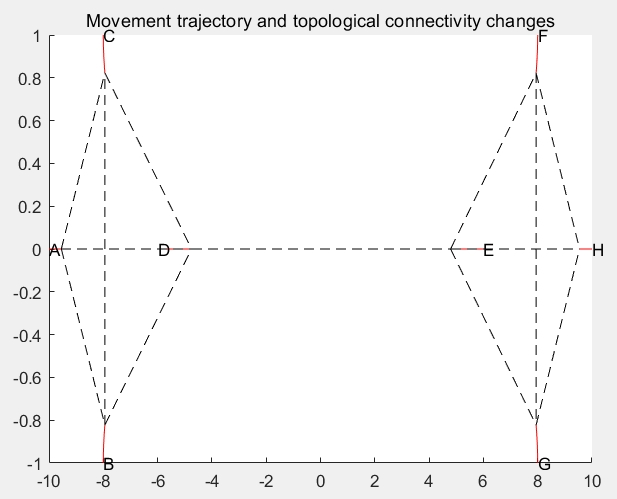
\includegraphics[width=\textwidth]{Image/type1.png}}
          % 加入对这列的图片说明
		\centerline{Topological situation 1}
	\end{minipage}
	\begin{minipage}{0.315\linewidth}
		\vspace{3pt}
		\centerline{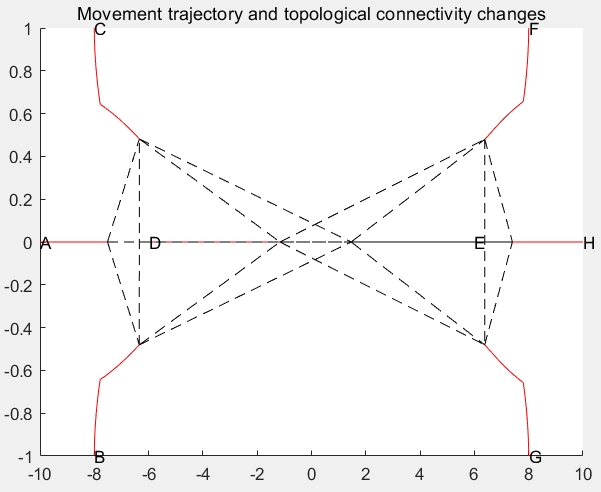
\includegraphics[width=\textwidth]{Image/type2.png}}
	 
		\centerline{Topological situation 2}
	\end{minipage}
	\begin{minipage}{0.32\linewidth}
		\vspace{3pt}
		\centerline{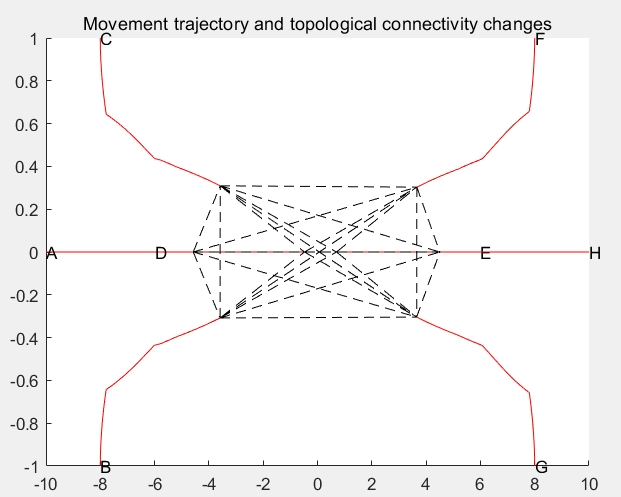
\includegraphics[width=\textwidth]{Image/type3.png}}
	 
		\centerline{Topological situation 3}
	\end{minipage}
 
	\caption{Different types of topological situations}

\end{figure}

链接插入:
\href{https://gitee.com/Racheus/me4409/tree/connection/}{https://gitee.com/Racheus/me4409/tree/connection/}

\newpage

\section{数学公式}
数学公式(行间、行内):

\begin{equation*}
    D(\mathcal{G})^T=\begin{bmatrix}
        1 & -1 & 0 & 0 & 0 & 0 & 0 & 0\\
        0 & 1 & -1 & 0 & 0 & 0 & 0 & 0\\
        0 & 0 & 1 & -1 & 0 & 0 & 0 & 0\\
        0 & 0 & 0 & 1 & -1 & 0 & 0 & 0\\
        0 & 0 & 0 & 0 & 1 & -1 & 0 & 0\\
        0 & 0 & 0 & 0 & 0 & 1 & -1 & 0\\
        0 & 0 & 0 & 0 & 0 & 0 & 1 & -1\\
    \end{bmatrix}
\end{equation*}

基于能量函数的方法,设计非线性连通保持控制器的过程如下:

将目标队形表述为$\tau_i \in \boldsymbol{R}^n$,$d_{ij} = \tau_i - \tau_j$。

记位移为$y_i = x_i(t) - \tau_i$,令$l_{ij}(t) = x_i(t)-x_j(t)$,则有$\lambda_{ij}(t) = l_{ij}(t) - d_{ij}$。

假设机器人的通讯半径为$\Delta$,定义能量函数
\begin{equation*}
    V_{ij}(\delta - \|d_{ij}\|,y) =
        \begin{cases}
        &\frac{\|\lambda_{ij}\|^2}{\Delta - \|d_{ij}\| - \|\lambda_{ij}\|}, \quad \text{if} \quad \{v_i,v_j\} \in E_d\\
        &0, \quad \text{otherwise}
        \end{cases}
\end{equation*}

求导,可以\textcolor{cherry}{设计控制器}:
\begin{equation*}
    u_i = \dot{x_i(t)} = -\sum_{j \in N_\mathcal{G}d(i)} \frac{
        2(\Delta - \|d_{ij}\| - \|\lambda_{ij}\|)}{(\Delta - \|d_{ij}\| - \|\lambda_{ij}\|)^2}(x_i(t) - x_j(t)-d_{ij})
\end{equation*}

\newpage
\section{表格环境}
表格环境{table}

\begin{table}[h]
    \centering
    \begin{tabular}{cc|c|c|c}
    \hline\hline
    \multicolumn{2}{c|}{}                                                                                                                           & \cellcolor[HTML]{ECF4FF}\textbf{48×48×48} & \cellcolor[HTML]{ECF4FF}\textbf{100×100×100} & \cellcolor[HTML]{ECF4FF}\textbf{216×216×216} \\ \hline
    \multicolumn{1}{c|}{}                                                                                      & \cellcolor[HTML]{FFFFD1}\textbf{1} & 0.998                                     & 10.419                                       & 134.256                                      \\ \cline{2-5} 
    \multicolumn{1}{c|}{}                                                                                      & \cellcolor[HTML]{FFFFD1}\textbf{2} & 0.554                                     & 6.269                                        & 90.683                                       \\ \cline{2-5} 
    \multicolumn{1}{c|}{\multirow{-3}{*}{\textbf{\begin{tabular}[c]{@{}c@{}}Solve\\ Time\\ (s)\end{tabular}}}} & \cellcolor[HTML]{FFFFD1}\textbf{4} & 0.326                                     & 4.220                                        & 75.198                                       \\ \hline
    \multicolumn{2}{c|}{内存占用(MB)}                                                                                                                   & 200.3                                     & 1012.55                                      & 10944.42                                     \\ \hline\hline
    \end{tabular}
    \end{table}


\end{document}
 